\documentclass[10pt, landscape]{article}
\usepackage[scaled=0.92]{helvet}
\usepackage{calc}
\usepackage{multicol}
\usepackage[a4paper,margin=3mm,landscape]{geometry}
\usepackage{amsmath,amsthm,amsfonts,amssymb}
\usepackage{color,graphicx,overpic}
\usepackage{hyperref}
\usepackage{newtxtext} 
\usepackage{enumitem}
\usepackage[table]{xcolor}
\usepackage{mathtools}
\setlist{nosep}
% for including images
\graphicspath{ {./images/} }

\pdfinfo{
  /Title (CS3223.pdf)
  /Creator (TeX)
  /Producer (pdfTeX 1.40.0)
  /Author (Jovyn Tan)
  /Subject (CS3223)
/Keywords (CS3223, nus,cheatsheet,pdf)}

% Turn off header and footer
\pagestyle{empty}

% redefine section commands to use less space
\makeatletter
\renewcommand{\section}{\@startsection{section}{1}{0mm}%
  {-1ex plus -.5ex minus -.2ex}%
  {0.5ex plus .2ex}%x
{\normalfont\large\bfseries}}
\renewcommand{\subsection}{\@startsection{subsection}{2}{0mm}%
  {-1explus -.5ex minus -.2ex}%
  {0.5ex plus .2ex}%
{\normalfont\normalsize\bfseries}}
\renewcommand{\subsubsection}{\@startsection{subsubsection}{3}{0mm}%
  {-1ex plus -.5ex minus -.2ex}%
  {1ex plus .2ex}%
{\normalfont\small\bfseries}}%
\makeatother

\renewcommand{\familydefault}{\sfdefault}
\renewcommand\rmdefault{\sfdefault}
%  makes nested numbering (e.g. 1.1.1, 1.1.2, etc)
\renewcommand{\labelenumii}{\theenumii}
\renewcommand{\theenumii}{\theenumi.\arabic{enumii}.}
\renewcommand\labelitemii{•}
\renewcommand\labelitemiii{•}

\definecolor{mathblue}{cmyk}{1,.72,0,.38}
\everymath\expandafter{\the\everymath \color{mathblue}}

% Don't print section numbers
\setcounter{secnumdepth}{0}

\setlength{\parindent}{0pt}
\setlength{\parskip}{0pt plus 0.5ex}
%% adjust spacing for all itemize/enumerate
\setlength{\leftmargini}{0.4cm}
\setlength{\leftmarginii}{0.4cm}
\setlength{\leftmarginiii}{0.2cm}
\setlist[itemize,1]{leftmargin=2mm,labelindent=1mm,labelsep=1mm}
\setlist[itemize,2]{leftmargin=4mm,labelindent=1mm,labelsep=1mm}
\setlist[itemize,3]{leftmargin=4mm,labelindent=1mm,labelsep=1mm}

% adding my commands
% tightcenter
\newenvironment{tightcenter}{%
  \setlength\topsep{0pt}
  \setlength\parskip{0pt}
  \begin{center}
    }{%
  \end{center}
}

% boxed
\newenvironment{tightbox}{%
  \setlength\topsep{0pt}
  \setlength\parskip{0pt}
  \begin{center}
    \begin{tabular}{|@{\hspace{\dimexpr\fboxsep+0.5\arrayrulewidth}}c@{\hspace{\dimexpr\fboxsep+0.5\arrayrulewidth}}|}
      \hline
    }
    {%
    \\ \hline
    \end{tabular}
  \end{center}
}

% fixed width box
\newenvironment{fixedbox}[1][0.7]{
  \setlength\topsep{0pt}
  \setlength\parskip{0pt}
  \begin{center}
    \begin{tabular}{|>{\centering\arraybackslash}m{#1\linewidth}|}
    \hline
  }{
  \\ \hline
  \end{tabular}
  \end{center}
}

% definition of a new term
\usepackage{soul}
\definecolor{paleyellow}{RGB}{251,243,218}
\newcommand{\definition}[2][]{\sethlcolor{paleyellow}\hl{\textbf{#2}} #1  $\rightarrow$}

% important note (attention)
\newcommand{\attention}{{\color{red}\textbf{! }}}


\makeatletter
\newcommand*{\xdashrightarrow}[2][]{%
  \mathrel{%
    \mathpalette{\da@xarrow{#1}{#2}{}\da@rightarrow{\,}{}}{}%
  }%
}
\newcommand*{\da@rightarrow}{\mathchar"0\hexnumber@\symAMSa 4B }
\newcommand*{\da@xarrow}[7]{%
  % #1: below
  % #2: above
  % #3: arrow left
  % #4: arrow right
  % #5: space left 
  % #6: space right
  % #7: math style 
  \sbox0{$\ifx#7\scriptstyle\scriptscriptstyle\else\scriptstyle\fi#5#1#6\m@th$}%
  \sbox2{$\ifx#7\scriptstyle\scriptscriptstyle\else\scriptstyle\fi#5#2#6\m@th$}%
  \sbox4{$#7\dabar@\m@th$}%
  \dimen@=\wd0 %
  \ifdim\wd2 >\dimen@
    \dimen@=\wd2 %   
  \fi
  \count@=2 %
  \def\da@bars{\dabar@\dabar@}%
  \@whiledim\count@\wd4<\dimen@\do{%
    \advance\count@\@ne
    \expandafter\def\expandafter\da@bars\expandafter{%
      \da@bars
      \dabar@ 
    }%
  }%  
  \mathrel{#3}%
  \mathrel{%   
    \mathop{\da@bars}\limits
    \ifx\\#1\\%
  \else
    _{\copy0}%
  \fi
  \ifx\\#2\\%
\else
  ^{\copy2}%
\fi
}%   
\mathrel{#4}%
}
\makeatother

% -----------------------------------------------------------------------

\begin{document}
\raggedright
\footnotesize
\begin{multicols*}{4}
  % multicol parameters
  \setlength{\columnseprule}{0.25pt}

  \begin{center}
    \fbox{%
      \parbox{0.8\linewidth}{\centering \textcolor{black}{
          {\Large\textbf{CS3223}}
        \\ \normalsize{AY22/23 SEM 2}}
        \\ {\footnotesize \textcolor{gray}{github/jovyntls}}
      }%
    }
  \end{center}

  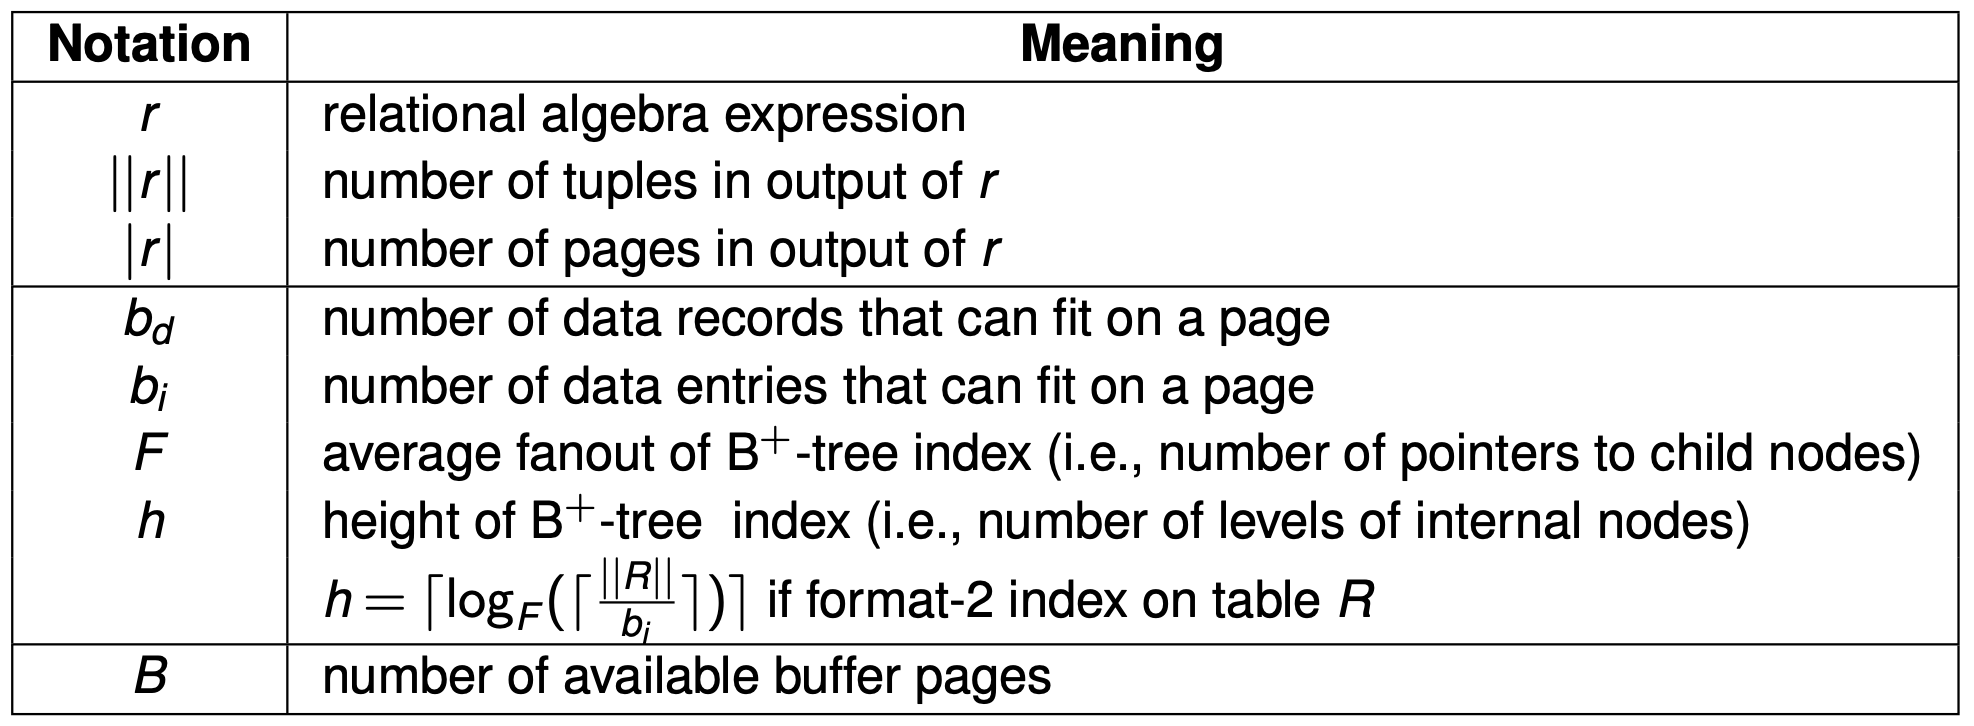
\includegraphics[width=0.97\linewidth]{cs3223-notation.png} 

  \textbf{Data entry formats}: \textbf{1.} actual data record; 
  \textbf{2.} \textbf{(k, RID)} - fixed length \texttt{(k, \textbf{$\bullet$})}; 
  \textbf{3.} \textbf{(k, RID-list)} - e.g. \texttt{(k, \{RID11, RID12\})}

  \section{04.1 SORTING}

  \begin{itemize}
    \item \definition{clustered index} order of data entries $\approx$ data records
      \begin{itemize}
        \item $\geq 1$ per relation; format 1 is always clustered
      \end{itemize}
  \end{itemize}

  \subsection{External Merge Sort}

  \begin{itemize}
    \item \definition{sorted run} sorted data records written to a file on disk
      \begin{enumerate}
        \item create temporary file $R_i$ for each $B$ pages of $R$ sorted
        \item merge: use $B-1$ pages for input, 1 page for output
      \end{enumerate}
    \item total I/O = $2N(\lceil \log_{B-1}(N_0) \rceil +1)$
      \begin{itemize}
        \item $2N$ to create $\lceil N/B \rceil $ sorted runs of $B$ pages each
        \item merging sorted runs: $2N \times \lceil \log_{B-1}N_0 \rceil $
      \end{itemize}
  \end{itemize}

  \subsubsection{optimisation with blocked I/O}

  \begin{itemize}
    \item sequential I/O - read/write in \textit{buffer blocks} of $b$ pages
    \item one block ($b$ pages) for output, remaining blocks for input
      \begin{itemize}
        \item number of runs merged per pass, $F = \lfloor \frac{B}{b} \rfloor -1$ 
        \item number of passes = $\lceil \log_F(N_0) \rceil +1$
      \end{itemize}
  \end{itemize}

  \subsubsection{Sorting with B$^+$-trees}

  \begin{itemize}
    \item when \textit{sort key is a prefix of the index key} of the B$^+$-tree
    \item sequentially scan leaf pages of B$^+$-tree
      \begin{itemize}
        \item for Format-2/3, use RID to retrieve data records
      \end{itemize}
  \end{itemize}

  \section{04.2 SELECTION: $\sigma_p(R)$}

  \begin{itemize}
    \item $\sigma_p(R)$ selects rows from relation $R$ satisfying predicate $p$
    \item \definition[of an access path]{selectivity} number of index \& data pages retrieved (more selective = fewer pages retrieved)
    \item \definition[for $Q$]{covering index $I$} if all attributes referenced in $Q$ are part of the key of $I$ 
      (\ildefinition{index-only plan}: no RID lookup) 
  \end{itemize}

  \subsection{Matching Predicates}

  \begin{itemize}
    \item \definition{term} of form $R.A \;\mathrm{op}\; c$ or $R.A_i \;\mathrm{op}\; R.A_j$
    \item \definition{conjunct} $\geq 1$ terms connected by $\lor$ (\ildefinition{disjunctive}: $>1$)
    \item \definition{CNF predicate} one or more conjuncts connected by $\land$
      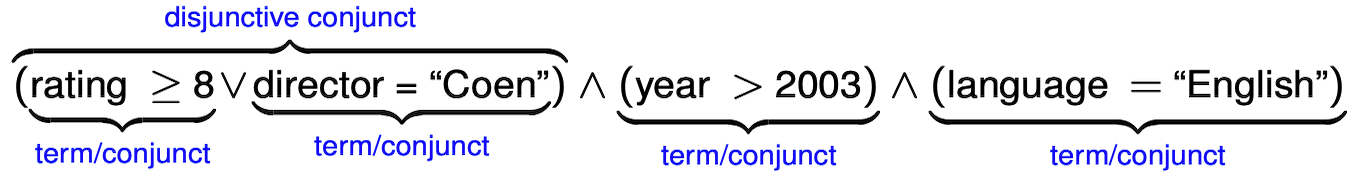
\includegraphics[width=0.95\linewidth]{cs3223-cnf-predicate.png} 
  \end{itemize}

  \textbf{B$^+$-tree matching predicates}

  \begin{itemize}
    \item for index $I=(K_1, K_2, \dots, K_n)$ and non-disjunctive CNF predicate $p$, $I$ matches $p$ if $p$ is of the form 
      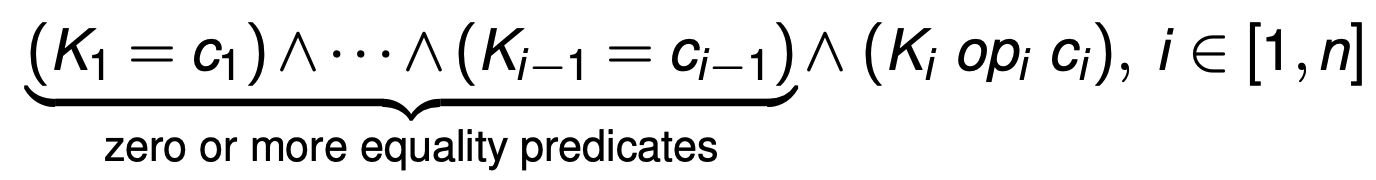
\includegraphics[width=0.9\linewidth]{cs3223-btree-matching-predicate.png} 
    \item matching index: matching records are in contiguous pages
  \end{itemize}

  \textbf{Hash index matching predicates}

  \begin{itemize}
    \item hash index $I$ matches $p$ if $p$ is of form  
      \\* \( {\displaystyle{ \quad\quad (K_1=c_1) \land (K_2=c_2) \land \dots \land (K_n=C_n) }} \) 
  \end{itemize}

  \subsection{Primary/Covered Conjuncts}

  \begin{itemize}
    \item \definition{primary conjuncts} subset of conjuncts that $I$ matches
      \begin{itemize}
        \item e.g. $p$ = \textcolor{blue}{(A $\geq$ 18) $\land$ (A $\leq$ 20)} $\land$ (W=65) 
          for $I=$ (A,W,H)
      \end{itemize}
    \item \definition{covered conjuncts} attribute appears in the key of $I$
      \begin{itemize}
        \item primary conjuncts $\subseteq$ covered conjuncts
      \end{itemize}
  \end{itemize}

  \subsection{Cost of Evaluation}

  let $p'$ = primary conjuncts of $p$, $\quad p_c$ = covered conjuncts of $p$

  \subsubsection{B$^+$-tree index evaluation of p}

  \begin{enumerate}
    \item navigate internal nodes to find first leaf page
      $ \text{cost}_{\text{internal}}= \lceil \log_F ( \lceil \frac{||R||}{b_{d \text{ or }i}} \rceil )\rceil \quad$ for format-1/otherwise
    \item scan leaf pages to access all qualifying data entries
      $\text{cost}_{\text{leaf}}=\lceil \frac{||\sigma_{p'}(R)||}{b_{d \text{ or }i}} \rceil\quad$ for format-1/otherwise
    \item retrieve qualified data records via RID lookups
      \\* $\text{cost}_{\text{RID}}=||\sigma_{p_c}(R)|| \quad$ or $0$ if $I$ is covering or format-1
      \begin{itemize}
        \item reduce cost with \textbf{clustered} data records (sort RIDs): 
          $\lceil\frac{||\sigma_{p_c}(R)||}{b_d}\rceil \leq \text{cost}_{RID} \leq \min\{||\sigma_{p_c}(R)||, |R|\}$
      \end{itemize}
  \end{enumerate}

  \subsubsection{hash index evaluation of p}

  \begin{itemize}
    \item \textbf{format-1}: $\quad$ cost to retrieve data records $ \geq \lceil\frac{||\sigma_{p'}(R)||}{b_d}\rceil $
    \item \textbf{format-2}: $\quad$ cost to retrieve data entries $ \geq \lceil\frac{||\sigma_{p'}(R)||}{b_i}\rceil $ 
      \\* cost to retrieve data records = $ \begin{cases} 0 \quad \text{if $$I$$ is a covering index,}\\
        ||\sigma_{p'}(R)||  \quad \text{otherwise}
      \end{cases} $
  \end{itemize}

  \section{05.1 PROJECTION $\pi_{A_1, \dots, A_m}(R)$}

  \begin{itemize}
    \item $\pi_L(R)$ eliminates duplicates, $\pi^*_L(R)$ preserves duplicates
    \item can \textbf{index scan} if index contains the attributes \textit{as a prefix}
  \end{itemize}

  \subsection{Sort-based approach}

  \textbf{cost analysis}

  \begin{enumerate}
    \item extract attributes: $|R|$ scan + $\vert \pi^*_L(R)\vert$ output temp result
    \item sort records: $2\vert \pi^*_L(R) \vert (\log_m(N_0) +1)$
    \item remove duplicates: $\vert \pi^*_L(R)\vert$ to scan records
  \end{enumerate}

  \textbf{optimised sort-based approach}

  \begin{enumerate}
    \item create sorted runs with projected attributes only
    \item merge sorted runs and remove duplicates
  \end{enumerate}
  \begin{itemize}
    \item if $B>\sqrt{|\pi^*_L(R)|}$, same I/O cost as hash-based approach
      \begin{itemize}
        \item $N_0 = \lfloor \frac{|R|}{B} \rfloor \approx \sqrt{|\pi^*_L(R)|}$ initial sorted runs 
        \item $\log_{B-1}(N_0) \approx 1$ merge passes
      \end{itemize}
  \end{itemize}

  \subsection{Hash-based approach}

  \begin{enumerate}
    \item \textbf{partitioning phase}: hash each tuple $t \in R$ to some $R_i$
      \begin{itemize}
        \item one buffer for input, $(B-1)$ buffers for output
        \item for each $t$: project attributes to form $t'$, hash $h(t')$ to one output buffer, flush output buffer to disk when full
      \end{itemize}
    \item \textbf{duplicate elimination} from each $\pi^*_L(R_i)$
      \begin{itemize}
        \item for each $R_i$: initialise in-mem hash table, hash each $t \in R_i$ to bucket $B_j$ with $h' \neq h$, insert if $t \not\in B_j$
        \item write tuples in hash table to results
      \end{itemize}
  \end{enumerate}

  \begin{itemize}
    \item \textbf{I/O cost} (no partition overflow): $|R| + 2|\pi^*_L(R)|$
      \begin{itemize}
        \item partitioning cost: $|R| + |\pi^*_L(R)|$
        \item duplicate elimination cost: $|\pi^*_L(R)|$
      \end{itemize}
    \item partition overflow: recursively apply partitioning
      \begin{itemize}
        \item to avoid, $B>$ size of hash table for $R_i$ = $\frac{|\pi^*_L(R)|}{B_1} \times f$
          \begin{itemize}
            \item  approximately $B> \sqrt{f\times |\pi^*_L(R)|}$
          \end{itemize}
      \end{itemize}
  \end{itemize}

  \section{05.2 JOIN $R \bowtie_\theta S$}

  $R$ = outer relation (smaller relation); $\quad S$ = inner relation

  \attention for \textbf{format-2} index, add cost of retrieving record

  \begin{itemize}
    \item \textbf{tuple-based} nested loop join: $|R| + ||R|| \times |S|$
    \item \textbf{page-based} nested loop join: $|R| + |R| \times |S|$
    \item \textbf{block nested loop join}: $|R| + ( \lceil \frac{|R|}{B-2} \rceil \times |S| )$, $\;\; |R|\leq|S|$
      \begin{itemize}
        \item 1 page output, 1 page input, $(B-2)$ pages to read $R$
        \item for each $(B-2)$ pages of $R$: for each $P_S$ of $S$: check r,s
      \end{itemize}
    \item \textbf{index nested loop join}: for joining $R.A_i = S.B_j$
      $|R| + ||R|| \times \left( \log_F(\lceil \frac{||S||}{b_d} \rceil ) + \lceil \frac{||S||}{b_d ||\pi_{B_j}(S)||} \rceil \right)$
  \end{itemize}

  \textbf{sort-merge join}

  \begin{itemize}
    \item sort R \& S: $2|R| (\log_m(N_R)+1) + 2|S| (\log_m(N_S)+1)$
    \item merge cost: $|R| + |S| \quad$ (worst case $|R| + ||R||\times|S|$)
  \end{itemize}

  \textbf{optimised sort-merge join}

  \begin{itemize}
    \item merge sorted runs until $B > N(R, i) + N(S, j)$; then join
    \item $3(|R|+|S|) = 2+1$ (for initial sorted runs + merging)
      \begin{itemize}
        \item if $B > \sqrt{2|S|}$, one pass to merge initial sorted runs
      \end{itemize}
  \end{itemize}

  \subsubsection{Grace hash join}

  for \textit{build relation} $R$ and \textit{probe relation} $S$,
  \begin{enumerate}
    \item \textbf{partition} $R$ and $S$ into  $k$ partitions each, $k=B-1$
      \begin{itemize}
        \item $\pi_A(R_i) \cap \pi_B(S_j) = \emptyset \quad \forall R_i, S_j, i \neq j$
        \item $R = R_1 \cup R_2 \cup \dots \cup R_k, \quad t \in R_i \iff h(t.A)=i$
      \end{itemize}
    \item \textbf{probing phase}: hash $r \in R_i$ with $h'(r.A)$ to table $T$;
      $\forall s \in S_i$, $r \in$ bucket $h'(s.B)$: output ($r,s$) if match
      \begin{itemize}
        \item $R \bowtie_{R.A=S.B} S = (R_1 \bowtie S_1) \cup \dots \cup (R_k \bowtie S_k)$
      \end{itemize} 
  \end{enumerate}

  \begin{itemize}
    \item \textbf{partition overflow} if $R_i$ cannot fit in memory: recurse
    \item I/O cost: $3(|R|+|S|) \quad$ (no partition overflow)
    \item $B > \frac{f \times |R|}{B-1} + 2$ (input \& output buffer) $\approx B > \sqrt{f\times |R|}$
      \begin{itemize}
        \item during probing, $B >$ size of each partition $+ 2$
      \end{itemize}
  \end{itemize}

  \subsection{adapting join algorithms}

  \begin{itemize}
    \item \textbf{multiple equality-join} conditions: $\scriptscriptstyle(R.A = S.A) \land (R.B=S.B)$
      \begin{itemize}
        \item index nested loop join: use index on some/all join attribs
        \item sort-merge join: sort on \textit{combination} of attributes
      \end{itemize}
    \item \textbf{inequality-join} conditions: $(R.A<S.A)$
      \begin{itemize}
        \item index nested loop join: requires B$^+$-tree index
        \item not applicable: sort-merge join, hash-based joins
      \end{itemize}
    \item \textbf{set operations}
      \begin{itemize}
        \item intersection: $\scriptscriptstyle R(A, B) \cap S(A, B) = \pi_{R.A, R.B} (R \bowtie_p S)$
        \item cross product: $R \times S = R \bowtie_{true} S$
        \item union/difference: duplicate elimination/slightly modified
      \end{itemize}
  \end{itemize}

  \section{06. QUERY EVALUATION}

  \begin{itemize}
    \item \textbf{aggregation}: maintain running information while table scan
      \begin{itemize}
        \item index scan if there is a covering index for the query
      \end{itemize}
    \item \textbf{group-by}: sort/hash to group by attributes then aggregate
      \begin{itemize}
        \item if group-by attributes are a B+tree prefix, just aggregate
      \end{itemize}
  \end{itemize}

  \textbf{materialised evaluation}

  \begin{itemize}
    \item evaluates bottom-up; materialise intermediate results to disk 
    \item $\times$ incurs I/O  $\;\checkmark$ simple implementation $\;\checkmark$ less memory
  \end{itemize}

  \textbf{pipelined evaluation} $\quad$ (top-down, demand-driven)

  \begin{itemize}
    \item interleaved execution of operators - pass output directly to parent operator - can switch execution to where it is needed
    \item \textit{blocking operator:} can't produce output until all input tuples received (grace hash \& sort-merge join, external mergesort)
  \end{itemize}

  \textbf{hybrid: pipelined evaluation with partial materialisation}

  \begin{itemize}
    \item materialise if repeatedly scanned (e.g. nested loop join)
  \end{itemize}

  \subsection{query plans}

  query: $\geq 1$ logical plans: implemented by $\geq 1$ physical plans

  \textbf{query plan trees}

  \begin{minipage}[c]{0.6\linewidth}\color{black}
    \begin{itemize}
      \item \definition{linear} $\geq$ 1 operand per join operation is a base relation
        (else \ildefinition{bushy})
      \item \definition{left-deep} every right join operand is a base relation
    \end{itemize}
  \end{minipage}
  \begin{minipage}[c]{0.36\linewidth}
    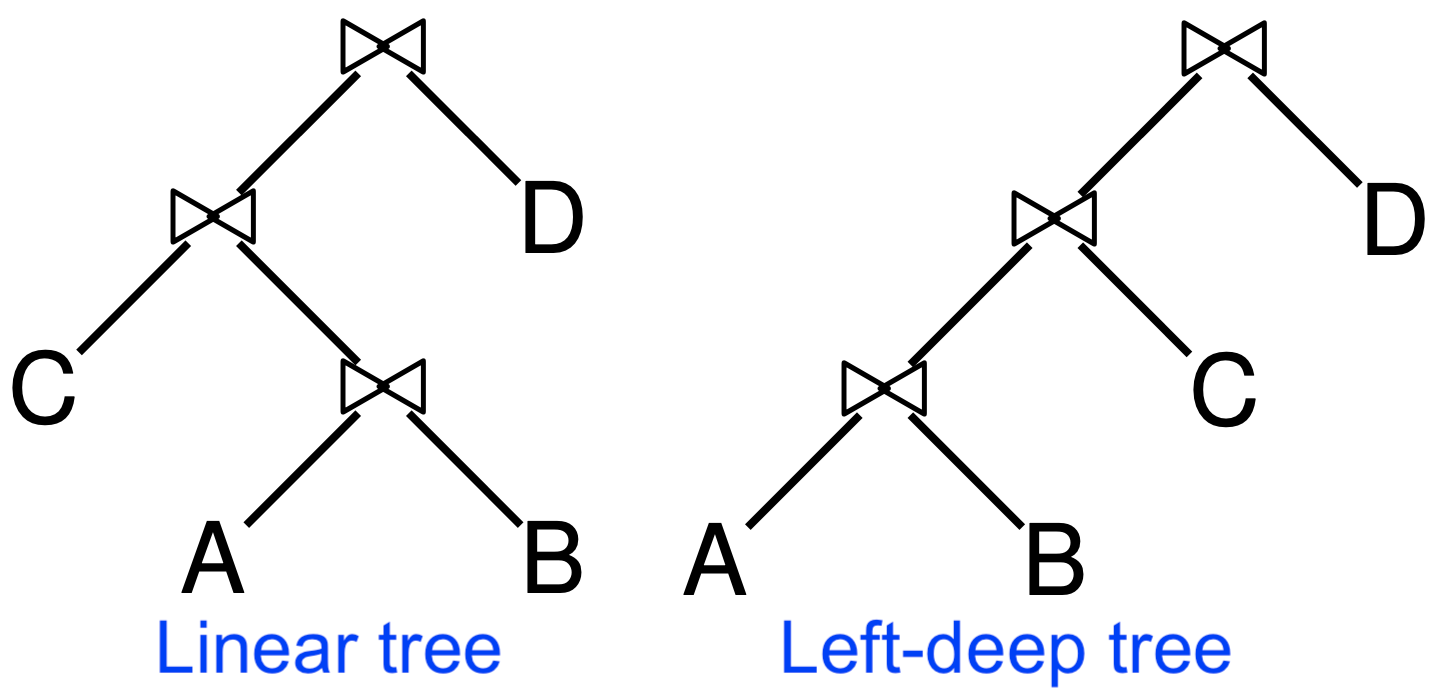
\includegraphics[width=\linewidth]{cs3223-query-plan-trees.png} 
  \end{minipage}

  \subsection{query optimisation}
  \begin{itemize}
    \item binary operators ($\bowtie, \times$) are \textbf{commutative \& associative}
      \begin{itemize}
        \item push selection and projection to operands first
      \end{itemize}
    \item DP query plan enumeration: use all optimal sub-plans to build overall plan (single-relation $\Rightarrow$ two-relation $\Rightarrow \dots$)
  \end{itemize}

  \begin{minipage}[c]{0.45\linewidth}
    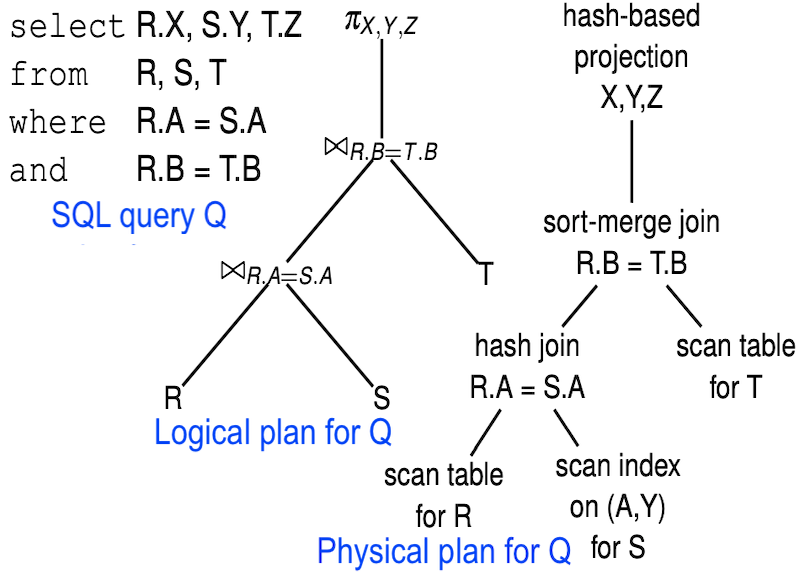
\includegraphics[width=\linewidth]{cs3223-query-plans.png} 
  \end{minipage}
  \begin{minipage}[c]{0.5\linewidth}
    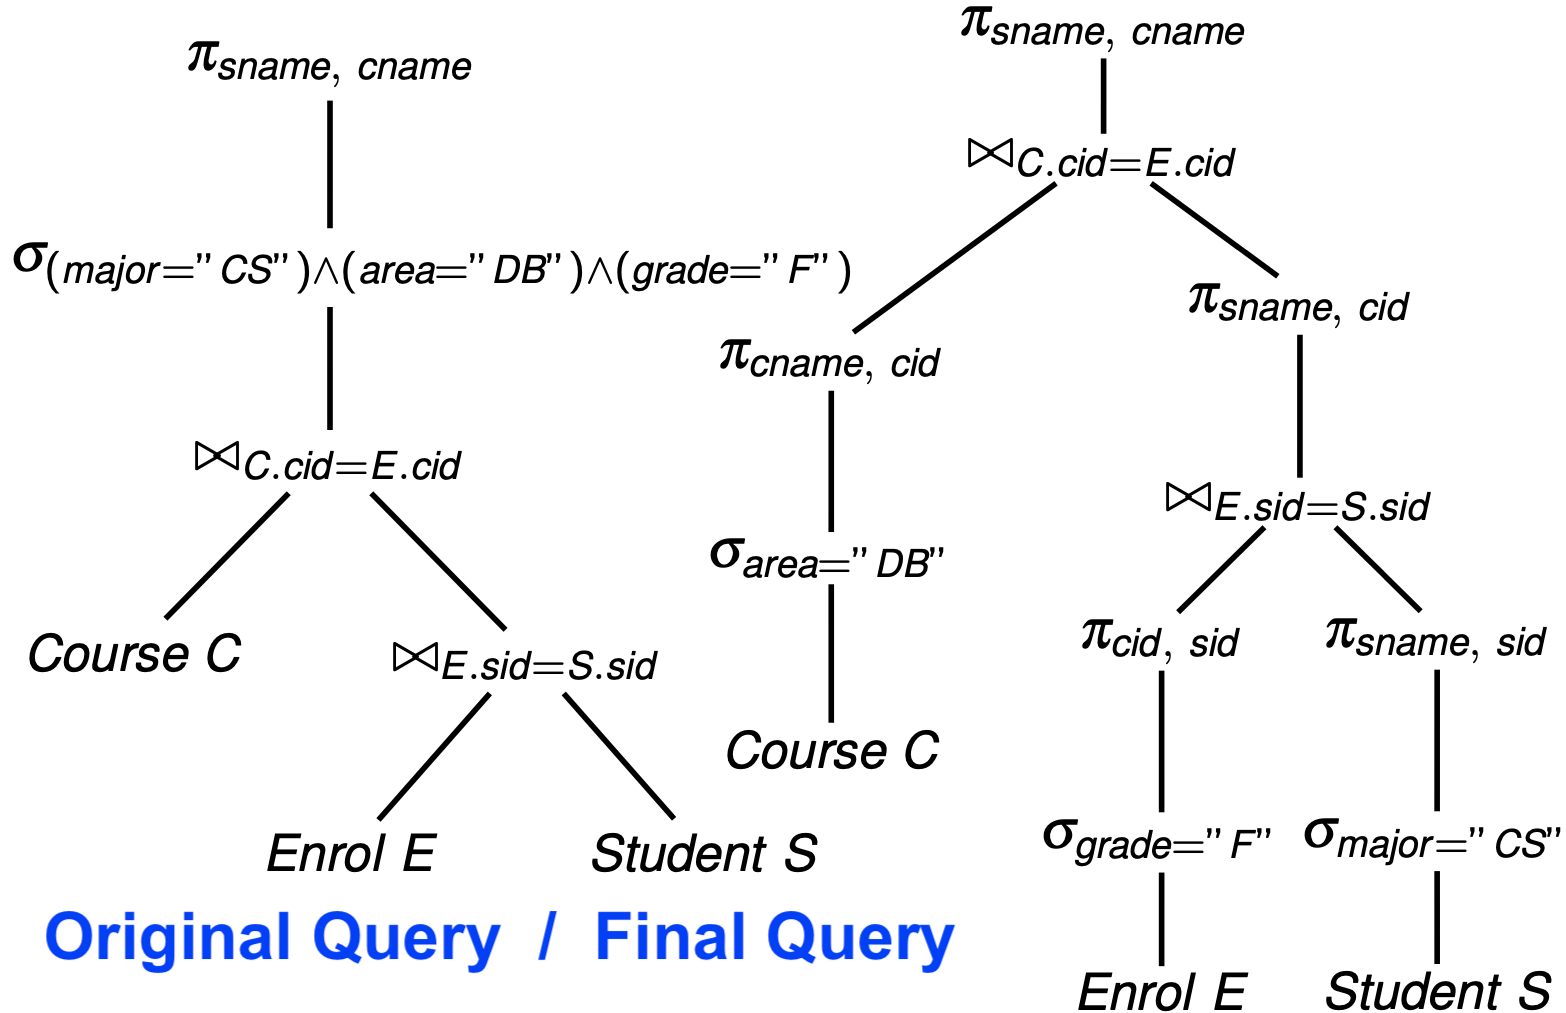
\includegraphics[width=\linewidth]{cs3223-query-optimisation-example.png} 
  \end{minipage}

  \textbf{System R Optimiser}

  \begin{itemize}
    \item enumerate only left-deep query plans; avoid cross-product query plans; consider early selections and projections
    \item DP + \textbf{sort order} $o_i$ of query plan output: $optPlan(S_i, o_i)$
  \end{itemize}

  \subsection{cost estimation}

  \begin{itemize}
    \item estimation assumptions
      \begin{enumerate}
        \item \textbf{uniformity} - of distribn of attr values
        \item \textbf{independence} - for distribn of values in different attrs
        \item \textbf{inclusion} - for $R \bowtie_{R.A=S.B}S$, if $||\pi_A(S)|| \leq ||\pi_B(S)||$, then $\pi_A(R) \subseteq \pi_B(S)$ 
          \\* $\Rightarrow$ every $R$ tuple joins with some $S$ tuple
      \end{enumerate}
    \item \textbf{size estimation} for query $q = \sigma_p(e)$,  $\quad p = t_1 \land \dots \land t_n$
      \begin{itemize}
        \item \definition{selectivity factor} fraction of tuples satisfying term
          \begin{itemize}
            \item aka \textit{reduction factor}, $rf(t_i) = \frac{||\sigma_t(e)||}{||e||}$
          \end{itemize}
        \item $||q|| \approx ||e|| \times \prod^n_{i=1}rf(t_i)$
        \item join selectivity: $rf(R.A=S.B) \approx \frac{1}{\max\{||\pi_A(R)||, ||\pi_B(S)||\}}$
      \end{itemize}
    \item \textbf{histogram estimation}
      \begin{itemize}
        \item \definition{equiwidth} $\approx$equal number of \textit{values} per bucket
        \item \definition{equidepth} $\approx$equal number of \textit{tuples} per bucket
        \item with \ildefinition{MCV}: keep a k/v pair of value/\#tuples
      \end{itemize}
  \end{itemize}

  \section{07. TRANSACTION MANAGEMENT}

  \begin{itemize}
    \item to ensure \definition[of transactions]{ACID properties} 
      \begin{enumerate}
        \item \textbf{atomicity} - either all or none of the actions happen
        \item \textbf{consistency} - if each txn is consistent, and the DB starts consistent, then the DB ends up consistent
        \item \textbf{isolation} - execution of one txn is isolated from other txn
        \item \textbf{durability} - if txn commits, its effects persist
      \end{enumerate}
  \end{itemize}

  \begin{itemize}
    \item \definition{view equivalent} same reads-from and final write
    \item \definition{view serialisable} view equiv to some serial schedule
    \item \definition{conflict} at least 1 write + different txns + same object
    \item \definition{conflict equivalent} all pairs of conflicting actions are ordered in the same way
  \end{itemize}

  \begin{itemize}
    \item \definition{conflict serialisable} conflict equivalent to a serial sched
      \begin{enumerate}
        \item acyclic conflict serialisability graph (node: committed txn, edge: precedes and conflicts with any action)
        \item conflict serialisable $\Rightarrow$ view serialisable
        \item view serialisable + no blind writes $\Rightarrow$ conflict serialisable
          \begin{itemize}
            \item \definition{blind write} did not read before write
          \end{itemize}
      \end{enumerate}
  \end{itemize}

  \textbf{anomalies} arise due to conflicting actions

  \begin{itemize}
    \item \textbf{dirty read} - due to WR conflicts
    \item \textbf{unrepeatable read} - due to RW conflict ($R_1,W_2,R_1$)
    \item \textbf{lost update} - due to WW conflict
    \item \textbf{phantom read} - re-executing a query on a search condition gives different results
      (prevent by predicate/index locking) 
  \end{itemize}

  \subsubsection{recovery}

  \begin{itemize}
    \item \definition{cascading abort} if $T_1$ reads from $T_2$, $T_1$ must abort when  $T_2$ aborts (for correctness)
    \item \definition{recoverable} if $T$ reads from $T'$, then $T$ commits after $T'$
      \begin{itemize}
        \item guarantees that committed txns will not be aborted
      \end{itemize}
    \item \definition{cascadeless} whenever $T_i$ reads from $T_j$, $Commit_j$ must precede this action
      \begin{itemize}
        \item all values read are produced by a committed transaction
      \end{itemize}
    \item \textbf{before-images}: log before action \& restore (must be strict)
    \item \definition{strict} for every $W_i(O)$ in $S$, $O$ is not read/written by another txn until $T_i$ either aborts or commits
    \item strict schedule $\Rightarrow$ cascadeless $\Rightarrow$ recoverable
  \end{itemize}

  \section{08. CONCURRENCY CONTROL}

  \subsection{Lock-based Concurrency Control}

  \subsubsection{2PL (Two Phase Locking)}

  \begin{itemize}
    \item may release locks any time
    \item once a txn releases a lock, it cannot request any more locks
      \begin{itemize}
        \item \textbf{growing/shrinking phase}: before/after releasing $1^{\text{st}}$ lock
      \end{itemize}
    \item prevents all anomalies, including phantom read
  \end{itemize}

  \subsubsection{Strict 2PL}

  \begin{itemize}
    \item \definition{Strict 2PL} txn must hold locks until it commits/aborts
    \item 2PL $\Rightarrow$ conflict serialisable
    \item strict 2PL $\Rightarrow$ strict \& conflict serialisable
  \end{itemize}

  \subsection{Lock Management}

  \subsubsection{deadlocks}

  \begin{itemize}
    \item \textbf{deadlock detection:} waits-for graph (WFG)
      \begin{itemize}
        \item nodes represent active txns
        \item edge $T_i \to T_j$ if $T_i$ is waiting for $T_j$ to release a lock
        \item WFG has a cycle $\Rightarrow$ deadlock
          \begin{itemize}
            \item abort one transaction and its edges from WFG
          \end{itemize}
      \end{itemize}
    \item \textbf{deadlock prevention:} older = higher priority
      \begin{itemize}
        \item \definition[policy]{wait-die} lower-priority aborts instead of waiting
          \begin{itemize}
            \item less aggressive; younger txns may keep aborting
          \end{itemize}
        \item \definition[policy]{wound-wait} (preemptive) higher- aborts lower-
          \begin{itemize}
            \item preemptive - can abort another txn
          \end{itemize}
          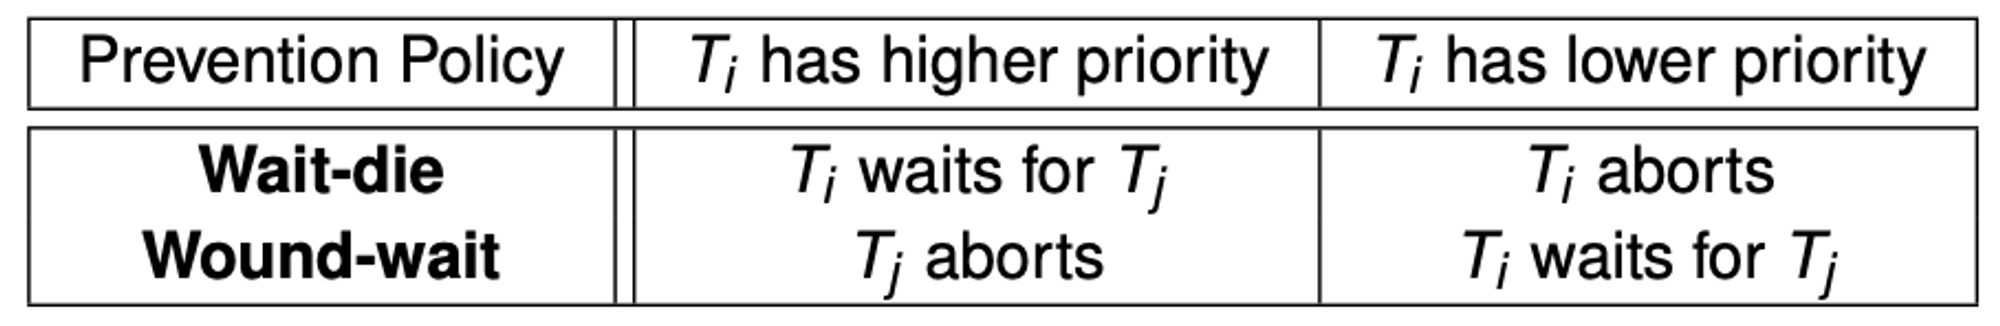
\includegraphics[width=0.95\linewidth]{cs3223-deadlock-prevention-policies} 
        \item restarted txn uses original timestamp to avoid starvation
      \end{itemize}
  \end{itemize}

  \subsubsection{lock conversion}

  \begin{itemize}
    \item increases concurrency; only in the growing phase
    \item \textbf{lock upgrade}, $UG_i(A)$: allowed if no other txn is holding a shared lock on $A$ and $T_i$ has not yet released any lock
      \begin{itemize}
        \item ensures serialisable schedule
      \end{itemize}
    \item \textbf{lock downgrade}, $DG_i(A)$: allowed if $T_i$ has not modified $A$ and has not released any lock
  \end{itemize}

  \subsection{ANSI SQL Isolation Levels}

  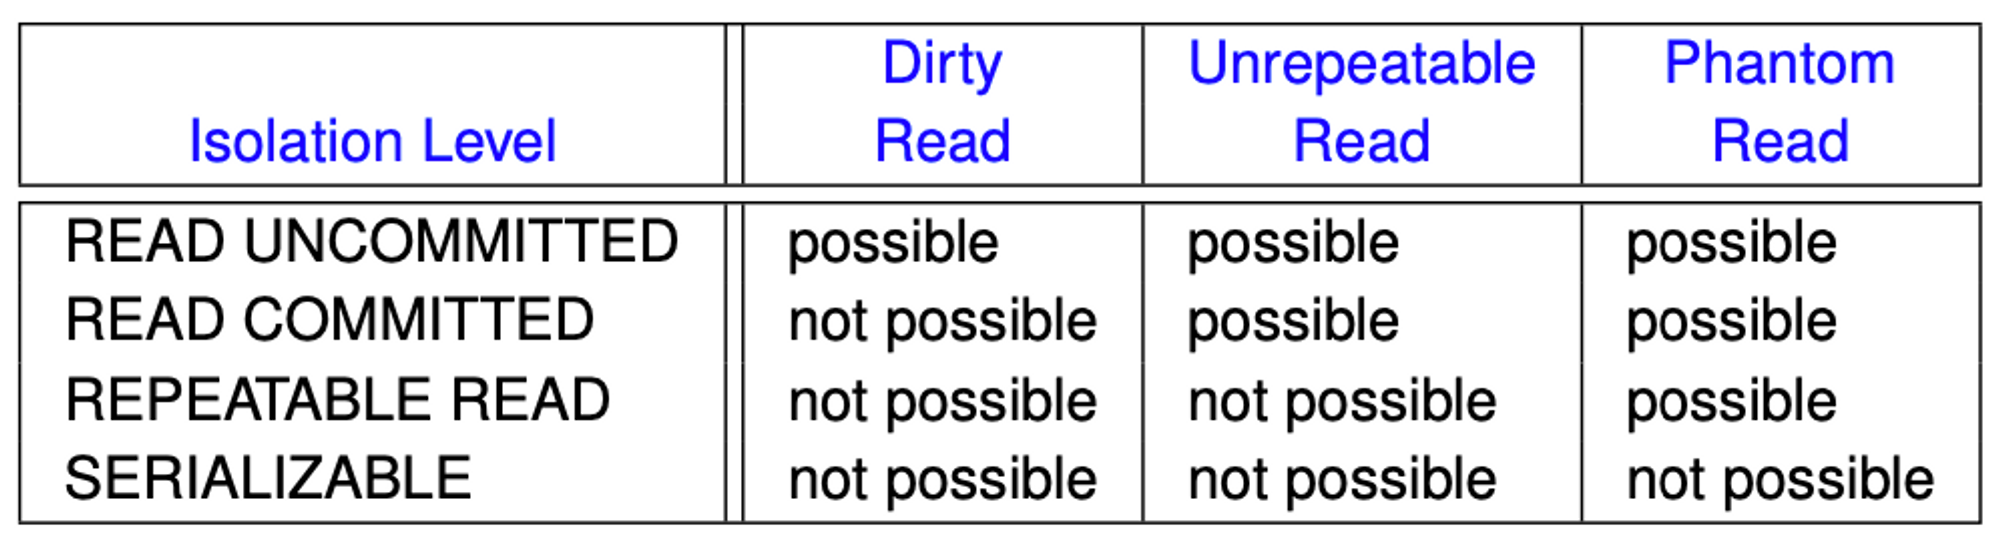
\includegraphics[width=0.95\linewidth]{cs3223-ansi-sql-isolation-levels.png} 
  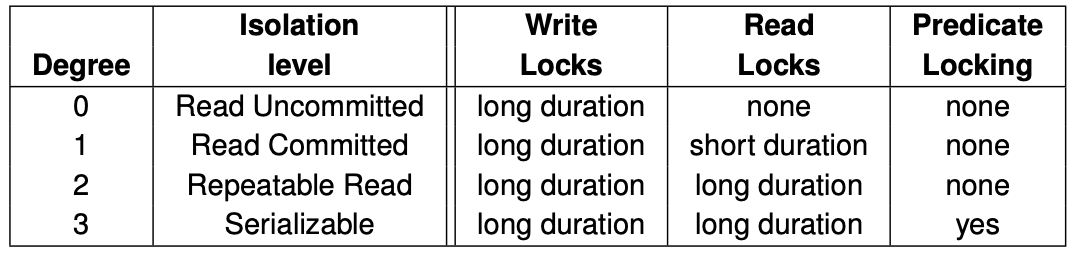
\includegraphics[width=0.95\linewidth]{cs3223-isolation-levels-lock-implementation.png} 

  \begin{itemize}
    \item \definition[lock]{short-duration} can be released before commit/abort
    \item \definition[lock]{long-duration} held until txn commits/aborts
  \end{itemize}

  \subsection{Locking Granularity}

  \begin{itemize}
    \item (coarsest/most granular) database > relation > page > tuple
    \item \definition[lock]{multi-granular} can request different granularity
      \begin{itemize}
        \item if $T$ holds lock mode $M$ on data granule $D$, then $T$ implicitly holds $M$ on data granules finer than $D$
      \end{itemize}
  \end{itemize}

  \textbf{$I$-lock (intention)}

  \begin{itemize}
    \item before acquiring any S-/X-lock on $G$, must acquire $I$-locks on granules coarser than $G$ in a \textit{top-down} manner
    \item can be shared with other $I$-locks
    \item $\times$ limited concurrency: S-lock is incompatible with  $I$-lock
  \end{itemize}

  \subsubsection{$IS$- and $IX$-lock (intention shared/exclusive)}

  \begin{itemize}
    \item acquire locks \textit{top-down}, release locks \textit{bottom-up}
      \begin{itemize}
        \item to obtain \textbf{S or IS lock}: must hold \textbf{IS or IX} lock on parent
        \item to obtain \textbf{X or IX lock}: must hold \textbf{IX} lock on parent
      \end{itemize}
  \end{itemize}

  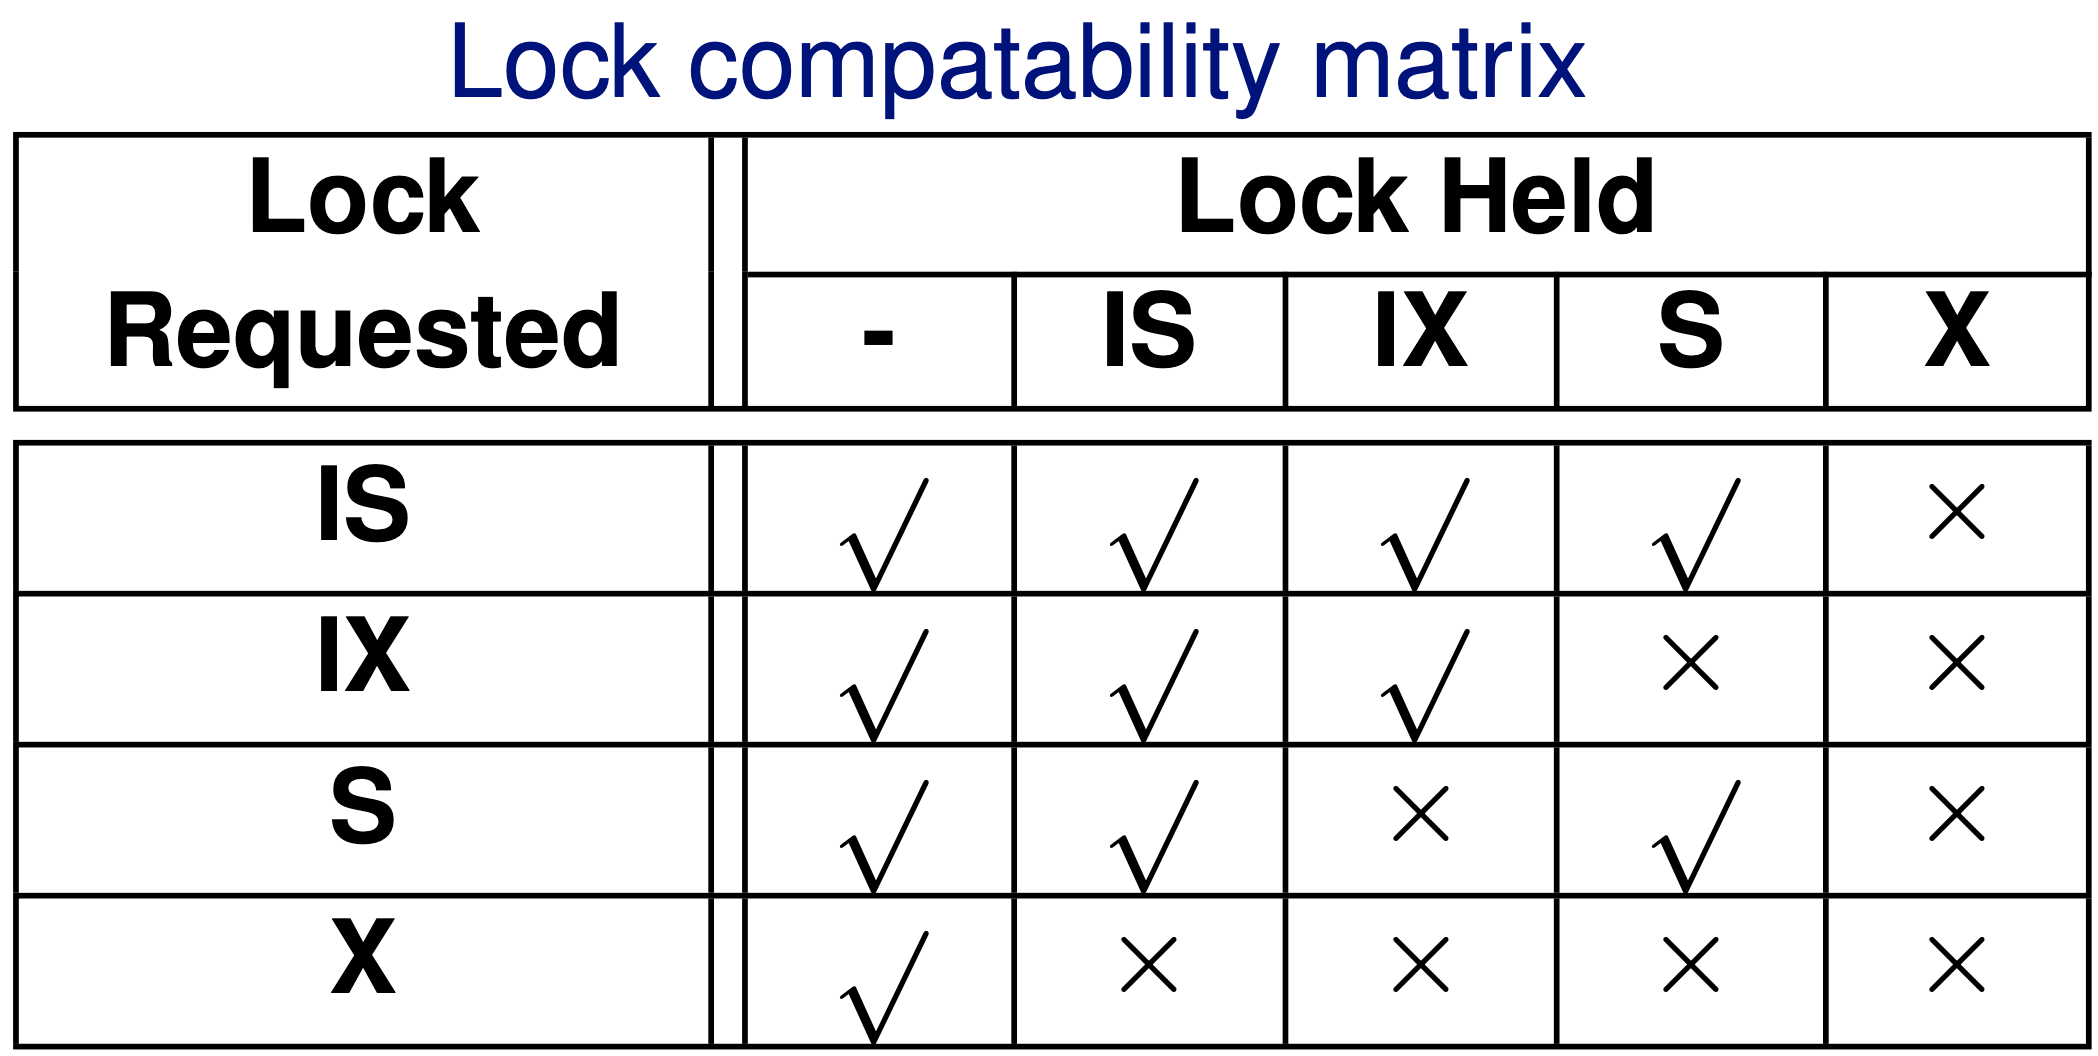
\includegraphics[width=0.5\linewidth]{cs3223-lock-compatibility-isix.png} 
  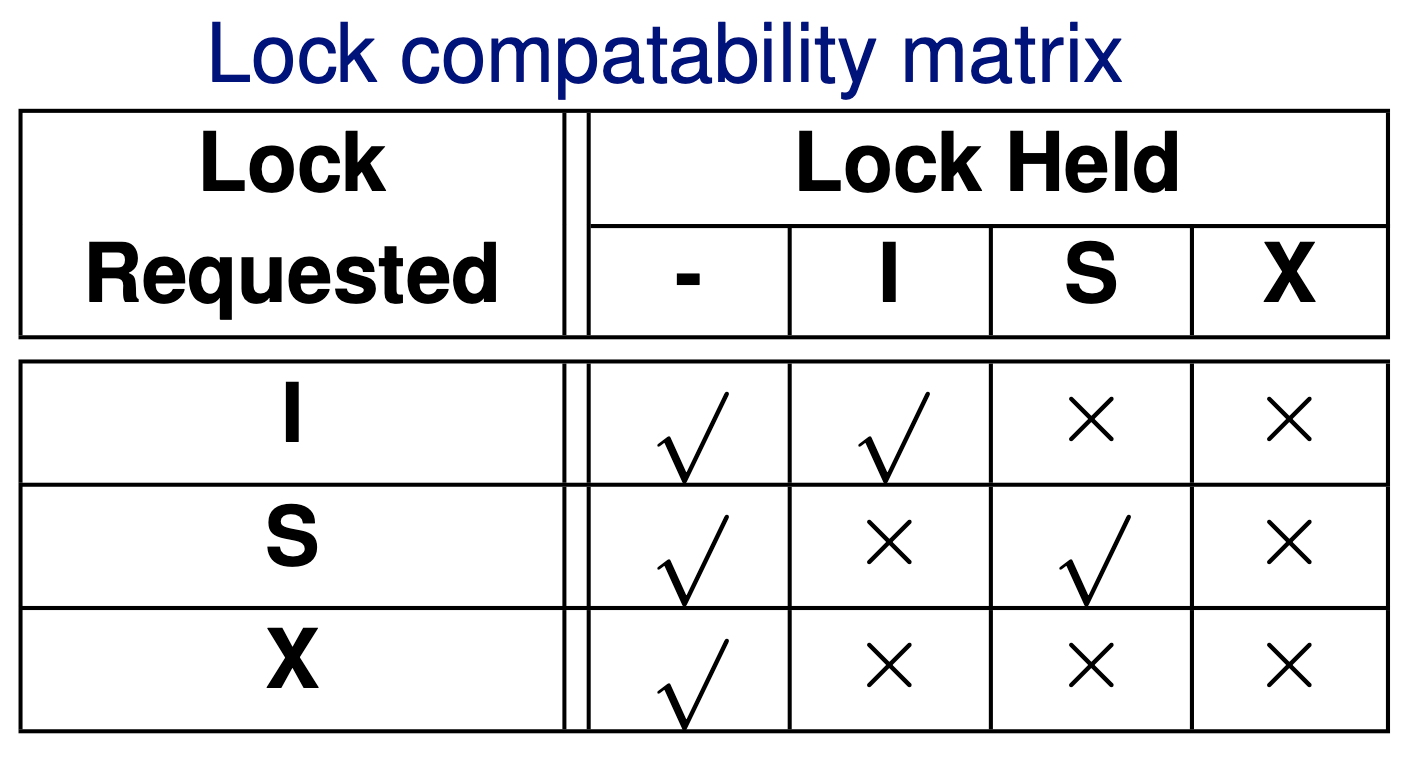
\includegraphics[width=0.45\linewidth]{cs3223-lock-compatibility-i-lock.png} 

  \section{09. MULTIVERSION CONCURRENCY CONTROL (MVCC)}

  \begin{itemize}
    \item maintain multiple versions of each object
      \begin{itemize}
        \item  $W_i(O)$ creates new version, $R_i(O)$ reads some version
      \end{itemize}
    \item $\checkmark$ read-only txns not blocked by update txns $\checkmark$ update txns not blocked by read-only txns $\checkmark$ read-only txns never aborted
    \item \definition[schedule]{multi-version} read can return \textit{any} version
    \item \definition{mono-version} always reads most recent version
    \item \definition[, $S \equiv_{mv} S'$]{multi-version view equivalent} same set of read-from relationships; $R_i(x_j) \in S \iff R_i(x_j) \in S'$
      \begin{itemize}
        \item final write doesn't matter (concept in monoversion only)
      \end{itemize}
    \item \definition[(MVSS)]{multi-version view serialisable} exists a \textit{serial mono-version schedule} that is multi-version view equivalent
      \begin{itemize}
        \item mono-version view serialisable $\Rightarrow$ MVSS
        \item VSS $\subseteq$ MVSS; $\quad$ VSS $\Rightarrow$ MVSS; $\quad$ MVSS $\not\Rightarrow$ VSS    
      \end{itemize}
  \end{itemize}

  \subsection{Snapshot Isolation}

  \begin{itemize}
    \item each txn $T$ sees a snapshot of the DB comprising updates by transactions that committed before $T$ starts
    \item \definition[txns]{concurrent} overlap, defined by start(T)/commit(T)
    \item \textbf{protocol}: $O_i$ is more recent if commit($T_i$) is later
      \begin{itemize}
        \item $W_i(O)$ creates version $i$ of $O$ 
        \item $R_i(O)$ reads either its latest $W_i(O)$ or the latest version of $O$ created by a txn that committed before start($T_i$)
      \end{itemize}
    \item \textbf{concurrent update property}: if multiple concurrent txn update the same object, only 1 commits (ensure serialisable)
      \begin{itemize}
        \item \ildefinition{FCW} (first committer wins): commit $\iff$ no committed concurrent txn on updated object
        \item \ildefinition{FUW} (first updater wins): acquire X-lock to update
          \begin{itemize}
            \item $T$ proceeds iff all concurrent $T'$ (previously holding the X-lock) aborts and $O$ has not been updated by any concurrent txn. $\quad/\quad$ else abort $T$
          \end{itemize}
      \end{itemize}
    \item \textbf{garbage collection}: if not read by any (active/future) txn
      \begin{itemize}
        \item delete $O_i$ if there exists a newer $O_j$ (commit($T_i$) < commit($T_j$)) such that for every active txn $T_k$ that started after commit($T_i$),  we have commit($T_j$) < start($T_k$)
      \end{itemize}
    \item \textbf{performance}: $\checkmark$ similar to READ\_COMMITTED but without \textit{lost update} or \textit{unrepeatable read} anomalies
      \begin{itemize}
        \item $\times$ $\not\Rightarrow$ serialisability (some non-serialisable executions)
          \begin{itemize}
            \item \textbf{write skew} anomaly: $\scriptscriptstyle R_1(x_0), R_2(y_0), W_1(y_1), W_2(x_2)$
            \item \textbf{read-only txn} anomaly: $\scriptscriptstyle T_3 \xdashrightarrow{rw} T_2 \xdashrightarrow{rw} T_1 \xrightarrow{wr} T_3$
          \end{itemize}
        \item $\times$ does not guarantee serialisability
      \end{itemize}
  \end{itemize}

  \subsubsection{Serialisable Snapshot Isolation (SSI)}

  \begin{itemize}
    \item ensures MVSS
    \item detect $T_i \xdashrightarrow{rw} T_j \xdashrightarrow{rw} T_k$ and abort one of $T_i, T_j, T_k$
      \begin{itemize}
        \item keeps track of \textbf{rw dependencies}; possible false positives
      \end{itemize}
  \end{itemize}

  \subsubsection{transactional dependencies: \texttt{ww}, \texttt{wr}, \texttt{rw}}

  \begin{itemize}
    \item \definition{immediate successor} no W(x) commits betw commits
    \item \textbf{dependency serialisation graph}, DSG
      \begin{itemize}
        \item nodes: (committed) transactions 
        \item edges: transactional dependencies, e.g. $T_i \xrightarrow{wr}T_j$
          \begin{itemize}
            \item $\dashrightarrow$/$\rightarrow$ for concurrent/non-concurrent
          \end{itemize}
      \end{itemize}
    \item if $S$ is a SI schedule that is not MVSS, then 
      \begin{itemize}
        \item there is \textit{at least one} cycle in $DSG(S)$
        \item for each cycle in $DSG(S)$, $\exists T_i, T_j, T_k$ such that
          \begin{itemize}
            \item $T_i \xdashrightarrow{rw} T_j \xdashrightarrow{rw} T_k$ exists
            \item $T_i$ and $T_k$ may be same txn (eg. write-skew anomaly)
          \end{itemize}
      \end{itemize}
  \end{itemize}

  \section{10. CRASH RECOVERY}

  \begin{itemize}
    \item \textbf{recovery manager} guarantees atomicity and durability
      \begin{itemize}
        \item undo: preserve atomicity (remove effects of aborts)
        \item redo: durability (re-install effects of commits)
      \end{itemize}
    \item \definition{steal policy} can write dirty page to disk before commit
    \item \definition{force policy} must write all dirty pages to disk at commit
  \end{itemize}
  \begin{minipage}[c]{0.57\linewidth}
    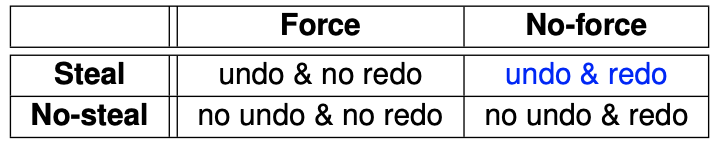
\includegraphics[width=\linewidth]{cs3223-steal-force-policy.png} 
  \end{minipage}
  \begin{minipage}[c]{0.4\linewidth}\color{black}
    \begin{itemize}
      \item no-steal: may run out of buffer pages
      \item force: incur random I/O
    \end{itemize}
  \end{minipage}

  \subsection{ARIES Recovery Algorithm}

  \begin{itemize}
    \item steal; no-force; assumes strict 2PL for concurrency control
  \end{itemize}

  \subsubsection{data structures}

  \begin{itemize}
    \item \textbf{log file} - sequential file of records in stable storage
    \item \textbf{transaction table (TT)} - 1 entry for each active txn
      \begin{itemize}
        \item (txn ID, last LSN, C/U status)
      \end{itemize}
    \item \textbf{dirty page table (DPT)} - 1 entry per dirty page in buffer pool
      \begin{itemize}
        \item (pageID, recLSN) = earliest log record that dirtied page
      \end{itemize}
    \item \textbf{log records}: (type, txn ID, prevLSN, other info)
      \begin{itemize}
        \item \textit{update} (\attention \textcolor{red}{redoable}): pageID, before-image, after-image
        \item \textit{compensation (CLR):} (\attention \textcolor{red}{redoable}) pageID, undoNextLSN (ULR's prevLSN), action to undo
          \begin{itemize}
            \item when update described by ULR is undone
          \end{itemize}
        \item \textit{commit}: force-write all records $\leq r$ to stable storage
          \begin{itemize}
            \item flush all log records for transaction to disk
          \end{itemize}
        \item \textit{abort:} create when txn is to be aborted
        \item \textit{end:} create when all processing for $T$ is completed
        \item \textit{checkpoint:} speed up recovery (scan from checkpoint)
      \end{itemize}
  \end{itemize}

  \subsubsection{implementing abort}

  \begin{itemize}
    \item \definition[protocol]{write-ahead logging (WAL)} do not flush an uncommitted update to the DB until the log record containing its before-image has been flushed to log
      \begin{itemize}
        \item each DB page contains \ildefinition{pageLSN} (LSN of latest update)
        \item before flushing page P, ensure all log records $\leq$ P.pageLSN have been flushed to disk
      \end{itemize}
  \end{itemize}

  \subsubsection{implementing commit}

  \begin{itemize}
    \item \definition[protocol]{force-at-commit} do not commit txn until the after-images of all its updated records are in stable storage
      \begin{itemize}
        \item \textit{commit LR}; txn is considered committed if its commit log record has been written to stable storage
      \end{itemize}
  \end{itemize}

  \subsubsection{implementing restart}

  \begin{enumerate}
    \item \ildefinition{analysis phase} - TT (active txns) \& DPT (superset of dirty)
      \begin{enumerate}
        \item initialise TT \& DPT (retrieve ECPLR from BCPLR)
        \item for each $r$ in log file in forward direction/chronological
          \begin{itemize}
            \item if \textit{end LR}, remove $T$ from TT; continue
            \item if \textit{redoable LR} for P and P not in DPT:
              \begin{itemize}
                \item create P's entry in DPT with recLSN=$r$.LSN
              \end{itemize}
            \item add or update entry for $T$ in TT: lastLSN = $r$.LSN
              \begin{itemize}
                \item if \textit{commit LR}: update status=C
              \end{itemize}
          \end{itemize}
      \end{enumerate}
    \item \ildefinition{redo phase} - restore DB to state at time of crash
      \begin{enumerate}
        \item start from \textbf{redoLSN} = smallest recLSN in DPT
        \item scan in forward direction for all \textit{redoable LR}
          \begin{enumerate}
            \item if \textit{not redoable} or \textcolor{blue}{NOT optimisation cond}: continue
            \item if P.pageLSN < $r$.LSN: ($r$ has not been installed)
              \begin{itemize}
                \item reapply logged action in $r$ to P
                \item update P.pageLSN = r.LSN
              \end{itemize}
            \item \textcolor{blue}{(optimisation)} else: recLSN $\leq$ r.LSN $\leq$ P.pageLSN
              \begin{itemize}
                \item update P in DPT: recLSN=P.pageLSN+1
              \end{itemize}
          \end{enumerate}
        \item create \textit{end LR} for all status=C in TT; remove entry
      \end{enumerate}
      \begin{itemize}
        \item \textcolor{blue}{optimisation} cond: (P $\not\in$ DPT) \textit{or} (DPT P.recLSN > r.LSN)
          \begin{itemize}
            \item update of $r$ has already been applied to P
          \end{itemize}
      \end{itemize}
    \item \ildefinition{undo phase} - abort \ildefinition{loser} txns (active at crash) in \textit{reverse}
      \begin{enumerate}
        \item initialise $L$ = set of lastLSN (status=U) from TT
          \begin{itemize}
            \item \texttt{update-L-and-TT(LSN)} := if LSN is not null, add to L; else create \textit{end LR} for T and remove T from TT
          \end{itemize}
        \item while $L \neq \emptyset$:
          \begin{enumerate}
            \item $r$ = largest lastLSN in L; delete $r$ from L
            \item if $r$ is \textit{update LR} for T on P:
              \begin{itemize}
                \item create \textit{CLR} $r_2$ with $r_2$.undoNextLSN=r.prevLSN
                \item update TT: T.lastLSN=$r_2$.LSN
                \item undo logged action and update P.pageLSN=$r_2$.LSN
                \item \texttt{update-L-and-TT}(r.prevLSN)
              \end{itemize}
            \item else if $r$ is \textit{CLR}: \texttt{update-L-and-TT}(r.undoNextLSN)
            \item else $r$ is \textit{abort LR}: \texttt{update-L-and-TT}(r.prevLSN)
          \end{enumerate}
      \end{enumerate}
  \end{enumerate}

  \subsubsection{normal transaction processing}

  \begin{itemize}
    \item \textbf{TT}: create new or update existing entry for $T$ (lastLSN)
      \begin{itemize}
        \item when $T$ commits, update status=C
        \item when end log record is generated, remove $T$'s entry
      \end{itemize}
    \item P is updated: update P.pageLSN = r.LSN
    \item P is updated \& not in DPT: create entry (recLSN=r.LSN)
    \item when P is flushed to disk: remove P's \textbf{DPT} entry
  \end{itemize}










\end{multicols*}

\end{document}
